\documentclass[dvipdfmx,11pt]{beamer}

%全体設定
%\AtBeginDvi{\special{pdf:tounicode 90ms-RKSJ-UCS2}}
\usepackage{ipsj}
\usepackage{color}
\usepackage{amssymb}
\usepackage{amsmath}
\usepackage{amsthm}
\usepackage{multirow,bigdelim}
\newcommand{\la}{\leftarrow}
\newcommand{\Lra}{\Longrightarrow}
\newcommand{\Lla}{\Longleftarrow}
\newcommand{\Llra}{\Longleftrightarrow}
\newcommand{\lra}{\longrightarrow}
\newcommand{\dd}{\mathop{..}}
\newcommand{\range}[2]{\{#1\dd#2\}}
\newcommand{\imp}{\Rightarrow}
\newcommand{\equ}{\Leftrightarrow}
\renewcommand{\labelenumi}{(\arabic{enumi})}
\newcommand{\alldiff}{\textrm{alldifferent}}
\newcommand{\Alldiff}{\alldiff(x_1,x_2,\ldots,x_n)}
\newcommand{\SAT}{{\tt SAT}}
\newcommand{\UNSAT}{{\tt UNSAT}}
\newcommand{\Dom}{{\it Dom}}
% \newcommand{\p}[2]{p(#1,#2)}
\newcommand{\dE}[2]{p(#1=#2)}
\newcommand{\lE}[2]{p(#1^{(#2)})}
\newcommand{\oE}[2]{p(#1\le#2)}


\title[ASPに基づく組合せ遷移ソルバーの実装方式に関する考察]{解集合プログラミングに基づく\\組合せ遷移ソルバーの実装方式に関する考察}
\author[山田 悠也,湊 真一,番原 睦則]{山田 悠也$^1$,湊 真一$^2$,番原 睦則$^1$}
\date{日本ソフトウェア科学会第38回大会}
\institute{1.名古屋大学 大学院情報学研究科 \\ 2.京都大学 大学院情報学研究科}

%% テンプレ 
\begin{comment}

%%%%%%%%%%%%%%%%%%%%%%%%%%%%%%%%%%%%%%%%%%%%%%%%%%
%% タイトル
%%%%%%%%%%%%%%%%%%%%%%%%%%%%%%%%%%%%%%%%%%%%%%%%%%
\begin{frame}\frametitle{}
\end{frame}

\end{comment}

%###########################################################
%# 本文 ####################################################
%###########################################################
\begin{document}

%%%%%%%%%%%%%%%%%%%%%%%%%%%%%%%%%%%%%%%%%%%%%%%%%%
%% タイトル 
%%%%%%%%%%%%%%%%%%%%%%%%%%%%%%%%%%%%%%%%%%%%%%%%%%
\begin{frame}\frametitle{}
  \titlepage
\end{frame}

%%%%%%%%%%%%%%%%%%%%%%%%%%%%%%%%%%%%%%%%%%%%%%%%%%
%% 組合せ遷移問題
%%%%%%%%%%%%%%%%%%%%%%%%%%%%%%%%%%%%%%%%%%%%%%%%%%
\begin{frame}\frametitle{組合せ遷移問題(Combinatorial Reconfiguration Problems)}

  \begin{alertblock}{}
    \alert{\bf 組合せ遷移問題}とは,
    基となる組合せ問題とその2つの実行可能解が与えられたとき,一方の実行可能解
    から他方の実行可能解へ,遷移制約を満たしつつ,
    実行可能解のみを経由して到達できるかを判定する問題.
  \end{alertblock}

  \begin{itemize}
    %\item 既存の組合せ問題の多くを組合せ遷移問題に拡張できる.
    \item 基となる問題が NP 完全であるとき,その遷移問題の多くは
      \alert{PSPACE完全}であることが知られている.
    \item 代表的な組合せ遷移問題
      \begin{itemize}
      \item 命題論理の充足可能性判定問題(SAT)の遷移問題~[Gopalan+ '09]
      \item 集合被覆問題の遷移問題~[Ito+ '11]
      \item グラフ点彩色問題の遷移問題~[Paul Bonsma+ '09]
      \end{itemize}
    \item 持続可能なシステムへの実用的応用が期待されている.
    \item 理論的な基盤が整備されつつある一方で,
          組合せ遷移問題の\alert{汎用的なソルバーの実践的な研究開発は始まったばかりである}.
  \end{itemize}
  %\begin{alertblock}{}%\centering
  %  本研究では,グラフ点彩色問題の遷移問題(\alert{$k$彩色遷移問
  %  題})をインスタンスとする.
  %\end{alertblock}
  
\end{frame}

%%%%%%%%%%%%%%%%%%%%%%%%%%%%%%%%%%%%%%%%%%%%%%%%%%
%% k彩色遷移問題
%%%%%%%%%%%%%%%%%%%%%%%%%%%%%%%%%%%%%%%%%%%%%%%%%%
\begin{frame}\frametitle{$k$彩色遷移問題}

  \begin{block}{$k$彩色遷移問題}
    \begin{itemize}
    \item 問題の入力として,グラフ点彩色問題とその二つの実行可能解
          (\structure{スタート状態}と\structure{ゴール状態})が与えられる.
    \item 遷移制約は「\structure{各遷移で色が変化する頂点はただ一つのみ}」である.
    \end{itemize}
  \end{block}

  \begin{exampleblock}{$k$彩色遷移問題の例}
    \begin{columns}
      \begin{column}{0.3\textwidth}
        \centering
        %%%%%%%%%%%%%%%%%%%%%%%%%%%%%%%%%%%%%%%%%%%%%%%%%%
% 実行例(t=0) (第6章で使う)
%%%%%%%%%%%%%%%%%%%%%%%%%%%%%%%%%%%%%%%%%%%%%%%%%%

\begin{tikzpicture}[scale=0.6]

  % 設定
  \tikzset{node/.style={circle,draw=black}}
 
  \definecolor{col_r}{RGB}{230,0,18}
  %\definecolor{col_b}{RGB}{0,104,183}
  \definecolor{col_b}{RGB}{51,51,179}
  \definecolor{col_y}{RGB}{255,251,0}
  \definecolor{col_g}{RGB}{0,96,0}
 
  % 補助線
  % \draw [help lines,blue] (0,0) grid (20,6);
 
  % node %
  \node[node, fill=col_r!70] (node1){\textbf{1}};
  \node[node, fill=col_b!70, right=of node1] (node2){\textbf{2}};
  \node[node, fill=col_y!70, below=of node1] (node3){\textbf{3}};
  \node[node, fill=col_g!70, below=of node2] (node4){\textbf{4}};
 
  \foreach \u / \v in {node1/node2, node2/node3, node2/node4, node3/node4}
  \draw (\u) -- (\v);
 \end{tikzpicture}
 
 %%%%%%%%%%%%%%%%%%%%%%%%%%%%%%%%%%%%%%%%%%%%%%%%%%%%%%%%%%
 %%% Local Variables:
 %%% mode: japanese-latex
 %%% TeX-master: paper.tex
 %%% End:
 
%        ステップ0($=\alpha$)
      \end{column}
      \begin{column}{0.05\textwidth}
        \textbf{$\longrightarrow$}
      \end{column}
      \begin{column}[]{0.3\textwidth}
        \centering
        \begin{tikzpicture}

 \tikzset{node/.style={circle,draw=black}}

 \definecolor{col_r}{RGB}{230,0,18}
 \definecolor{col_b}{RGB}{51,51,179}
 \definecolor{col_y}{RGB}{255,251,0}
 \definecolor{col_g}{RGB}{0,96,0}

 \node[node, fill=col_r!70] (node1){\textbf{1}};
 \node[node, fill=col_g!70, right=of node1] (node2){\textbf{2}};
 \node[node, fill=col_b!70, below=of node1] (node3){\textbf{3}};
 \node[node, fill=col_y!70, below=of node2] (node4){\textbf{4}};

 \foreach \u / \v in {node1/node2, node1/node3, node1/node4, node2/node3, node2/node4, node3/node4}
 \draw (\u) -- (\v);

\end{tikzpicture}
%        ステップ1
      \end{column}
      \begin{column}{0.05\textwidth}
        \textbf{$\longrightarrow$}
      \end{column}
      \begin{column}{0.3\textwidth}
        \centering
        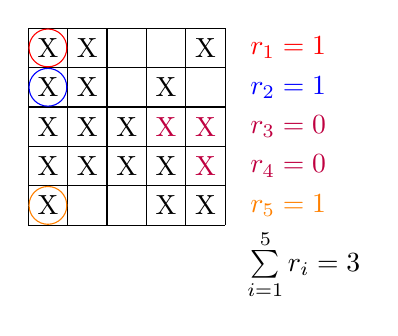
\begin{tikzpicture}
 \draw (0,0)--(2.5,0);
 \draw (0,0.5)--(2.5,0.5);
 \draw (0,1.0)--(2.5,1.0);
 \draw (0,1.5)--(2.5,1.5);
 \draw (0,2.0)--(2.5,2.0);
 \draw (0,2.5)--(2.5,2.5);
 \draw (0,0)--(0,2.5);
 \draw (0.5,0)--(0.5,2.5);
 \draw (1.0,0)--(1.0,2.5);
 \draw (1.5,0)--(1.5,2.5);
 \draw (2.0,0)--(2.0,2.5);
 \draw (2.5,0)--(2.5,2.5);
 \node (X) at (0.25,0.25) {X};
 \draw [orange] (0.25,0.25) circle[radius = 0.24];
 \node (X) at (0.25,0.75) {X};
 \node (X) at (0.25,1.25) {X};
 \node (X) at (0.25,1.75) {X};
 \draw [blue] (0.25,1.75) circle[radius = 0.24];
 \node (X) at (0.25,2.25) {X};
 \draw [red] (0.25,2.25) circle[radius = 0.24];
 \node (X) at (0.75,2.25) {X};
 \node (X) at (0.75,0.75) {X};
 \node (X) at (0.75,1.25) {X};
 \node (X) at (0.75,1.75) {X};
 \node (X) at (1.25,0.75) {X};
 \node (X) at (1.25,1.25) {X};
 \node (X) at (1.75,0.25) {X};
 \node (X) at (1.75,0.75) {X};
 \node (X) at (1.75,1.25) {\color{purple}X};
 \node (X) at (1.75,1.75) {X};
 \node (X) at (2.25,0.25) {X};
 \node (X) at (2.25,0.75) {\color{purple}X};
 \node (X) at (2.25,1.25) {\color{purple}X};
 \node (X) at (2.25,2.25) {X};
 \node (A) at (3.30,2.25) {\color{red}$r_{1} = 1$};
 \node (B) at (3.30,1.75) {\color{blue}$r_{2} = 1$};
 \node (M) at (3.30,1.25) {\color{purple}$r_{3} = 0$};
 \node (M) at (3.30,0.75) {\color{purple}$r_{4} = 0$};
 \node (C) at (3.30,0.25) {\color{orange}$r_{5} = 1$};
 \node (D) at (3.50,-0.50) {$\sum\limits_{i=1}^{5}r_{i}=3$};
\end{tikzpicture}
%        ステップ2($=\beta$)
      \end{column}
    \end{columns}
  \end{exampleblock}
  
\end{frame}

%%%%%%%%%%%%%%%%%%%%%%%%%%%%%%%%%%%%%%%%%%%%%%%%%%
%% ASP
%%%%%%%%%%%%%%%%%%%%%%%%%%%%%%%%%%%%%%%%%%%%%%%%%%
\begin{frame}\frametitle{解集合プログラミング(Answer Set Programming; ASP)}

  \begin{itemize}
    \item ASP の言語は一般拡張選言プログラムに基づく.
    \item ASPシステムは安定モデル理論~[Gelfond and Lifschitz '88] に基づく
          解集合を計算するシステムである.
    \item 近年,SAT技術の応用により高速なASPシステムが実現し, 
          システム検証やプランニングなどの様々な分野での実用的応用が拡大している.
  \end{itemize}

  \begin{alertblock}{組合せ遷移問題に対してASPを用いる利点}
    \begin{itemize}
      \item ASPの高い表現力により,記号制約を簡潔に記述できる.
      \item インクリメンタルASP解法により,同様の探索失敗を避けるために獲得した学習節を保持することで,遷移問題に対する効率的な解探索が可能である.
    \end{itemize}
  \end{alertblock}
  
\end{frame}

%%%%%%%%%%%%%%%%%%%%%%%%%%%%%%%%%%%%%%%%%%%%%%%%%%
%% ASP
%%%%%%%%%%%%%%%%%%%%%%%%%%%%%%%%%%%%%%%%%%%%%%%%%%
\begin{frame}\frametitle{ASP の基本的な構文}

  一般拡張選言プログラムのサブクラスである
  論理プログラム\footnote{標準論理プログラムを指す.}について説明する.

  \begin{itemize}
    \item \structure{論理プログラム}とは,以下の形式の
          \structure{ルール}の有限集合である.
          \begin{block}{}
            \centering
            $a_0$ \code{:-} $a_1, \dots, a_m,$ \code{not} $a_{m+1}, \dots,$ \code{not} $a_{n}$
          \end{block}
          \begin{itemize}
            \item $0 \le m \le n$であり,各$a_i$はアトム,\code{not}はデフォルトの否定,
                  ``\code{,}''は連言を表す.\code{:-}の左側をヘッド,右側をボディと呼ぶ.
            \item 直感的な意味は,「$a_1, \dots, a_m,$が成り立ち,$a_{m+1}, \dots, a_{n}$
                  が成り立たないのであれば$a_{0}$は成り立つ」である.
          \end{itemize}       
    \item ボディが空のルールを\structure{ファクト}と呼び,\code{:-}を省略できる.
          \begin{itemize}
            \item ヘッドが常に成り立つことを意味する.
          \end{itemize}
    \item ヘッドが空のルールを\structure{一貫性制約}と呼ぶ.例えば,
          \code{:-} $a_1,$ \code{not} $a_2$は,$a_1$が成り立つなら$a_2$が
          成り立つことを意味する.
  \end{itemize}
  
\end{frame}

%%%%%%%%%%%%%%%%%%%%%%%%%%%%%%%%%%%%%%%%%%%%%%%%%%
%% ASP
%%%%%%%%%%%%%%%%%%%%%%%%%%%%%%%%%%%%%%%%%%%%%%%%%%
\begin{frame}\frametitle{ASP の拡張構文}

  \begin{itemize}
    \item \structure{選択子}は
          \begin{center}
            \code{\{} $a_0$ \code{;} $\dots$ \code{;} $a_{m}$ \code{\}}
          \end{center}
          の形式で記述される.
          \begin{itemize}
            \item アトムの集合$\{ a_0, \dots, a_m\}$の任意の部分集合が成り立つことを
                  意味する.
          \end{itemize}
    \item \structure{個数制約}は
          \begin{center}
            $lb$ \code{\{} $a_0$ \code{;} $\dots$ \code{;} $a_{m}$ \code{\}} $ub$
          \end{center}
          の形式で記述される.
          \begin{itemize}
            \item $a_0, \dots, a_m$のうち,$lb$個以上$ub$個以下が成り立つことを意味する.
          \end{itemize}
  \end{itemize}
  
\end{frame}

%%%%%%%%%%%%%%%%%%%%%%%%%%%%%%%%%%%%%%%%%%%%%%%%%%
%% 研究目的
%%%%%%%%%%%%%%%%%%%%%%%%%%%%%%%%%%%%%%%%%%%%%%%%%%
\begin{frame}\frametitle{研究目的}

  \begin{alertblock}{目的}
    ASP技術を活用し,大規模な組合せ遷移問題を効率よく解くシステムを実現する.
  \end{alertblock}

  \begin{block}{研究内容}
    \begin{enumerate}
    \item 組合せ遷移問題に対して,有界組合せ遷移を提案した.
    \item 有界組合せ遷移に基づき組合せ遷移問題を解く2つのソルバーを提案した.
    \item $k$彩色遷移問題を解く2種類の符号化を提案した.
    \item 独自に作成したベンチマーク問題を用い,ソルバー及び符号化の評価実験を行った.
    \end{enumerate}
  \end{block}

\end{frame}

%%%%%%%%%%%%%%%%%%%%%%%%%%%%%%%%%%%%%%%%%%%%%%%%%%
%% 有界組合せ遷移
%%%%%%%%%%%%%%%%%%%%%%%%%%%%%%%%%%%%%%%%%%%%%%%%%%
\begin{frame}\frametitle{有界組合せ遷移}

  \begin{alertblock}{}
    \alert{\bf 有界組合せ遷移}とは,
    組合せ遷移問題に対してステップ長$\ell$を
    与え到達可能性を検査するものである.
  \end{alertblock}

  \begin{itemize}
    \item 与えられた組合せ遷移問題に対して,
          \structure{長さ$\ell$の遷移系列が存在するか}を解く.
    \item 制限された長さで系列が存在しない場合,長さを1増加させ
          再度問題を解く.
    \item 有界組合せ遷移は到達可能な遷移系列を探すのみで,
          到達不能の証明は行わない.
          \begin{itemize}
            \item ただし,適切な$\ell$の上限値を与えることで到達不能の
                  証明も行える.
          \end{itemize}
    \item 仮に遷移系列が存在する場合,得られた遷移系列は組合せ遷移問題の解の中で
          最短のものである.
  \end{itemize}

\end{frame}

%%%%%%%%%%%%%%%%%%%%%%%%%%%%%%%%%%%%%%%%%%%%%%%%%%
%% 有界組合せ遷移
%%%%%%%%%%%%%%%%%%%%%%%%%%%%%%%%%%%%%%%%%%%%%%%%%%
\begin{frame}\frametitle{有界組合せ遷移の例}

  \begin{enumerate}
    \item $\ell = 0$とする.
    \item $\ell = 0$のとき,到達不能である.
    \item $\ell = \ell + 1$とする.
    \item $\ell = 1$のとき,到達不能である.
    \item $\ell = \ell + 1$とする.
    \item $\ell = 2$のとき,到達可能である. 
  \end{enumerate}

  \begin{exampleblock}{$k$彩色遷移問題の例}
    \begin{columns}
      \begin{column}{0.3\textwidth}
        \centering
        %%%%%%%%%%%%%%%%%%%%%%%%%%%%%%%%%%%%%%%%%%%%%%%%%%
% 実行例(t=0) (第6章で使う)
%%%%%%%%%%%%%%%%%%%%%%%%%%%%%%%%%%%%%%%%%%%%%%%%%%

\begin{tikzpicture}[scale=0.6]

  % 設定
  \tikzset{node/.style={circle,draw=black}}
 
  \definecolor{col_r}{RGB}{230,0,18}
  %\definecolor{col_b}{RGB}{0,104,183}
  \definecolor{col_b}{RGB}{51,51,179}
  \definecolor{col_y}{RGB}{255,251,0}
  \definecolor{col_g}{RGB}{0,96,0}
 
  % 補助線
  % \draw [help lines,blue] (0,0) grid (20,6);
 
  % node %
  \node[node, fill=col_r!70] (node1){\textbf{1}};
  \node[node, fill=col_b!70, right=of node1] (node2){\textbf{2}};
  \node[node, fill=col_y!70, below=of node1] (node3){\textbf{3}};
  \node[node, fill=col_g!70, below=of node2] (node4){\textbf{4}};
 
  \foreach \u / \v in {node1/node2, node2/node3, node2/node4, node3/node4}
  \draw (\u) -- (\v);
 \end{tikzpicture}
 
 %%%%%%%%%%%%%%%%%%%%%%%%%%%%%%%%%%%%%%%%%%%%%%%%%%%%%%%%%%
 %%% Local Variables:
 %%% mode: japanese-latex
 %%% TeX-master: paper.tex
 %%% End:
 
        $t=0$
      \end{column}
      \begin{column}{0.05\textwidth}
        \textbf{$\longrightarrow$}
      \end{column}
      \begin{column}[]{0.3\textwidth}
        \centering
        \begin{tikzpicture}

 \tikzset{node/.style={circle,draw=black}}

 \definecolor{col_r}{RGB}{230,0,18}
 \definecolor{col_b}{RGB}{51,51,179}
 \definecolor{col_y}{RGB}{255,251,0}
 \definecolor{col_g}{RGB}{0,96,0}

 \node[node, fill=col_r!70] (node1){\textbf{1}};
 \node[node, fill=col_g!70, right=of node1] (node2){\textbf{2}};
 \node[node, fill=col_b!70, below=of node1] (node3){\textbf{3}};
 \node[node, fill=col_y!70, below=of node2] (node4){\textbf{4}};

 \foreach \u / \v in {node1/node2, node1/node3, node1/node4, node2/node3, node2/node4, node3/node4}
 \draw (\u) -- (\v);

\end{tikzpicture}
        $t=1$
      \end{column}
      \begin{column}{0.05\textwidth}
        \textbf{$\longrightarrow$}
      \end{column}
      \begin{column}{0.3\textwidth}
        \centering
        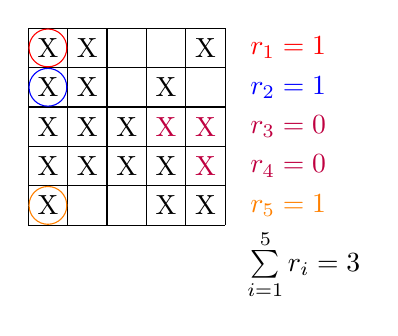
\begin{tikzpicture}
 \draw (0,0)--(2.5,0);
 \draw (0,0.5)--(2.5,0.5);
 \draw (0,1.0)--(2.5,1.0);
 \draw (0,1.5)--(2.5,1.5);
 \draw (0,2.0)--(2.5,2.0);
 \draw (0,2.5)--(2.5,2.5);
 \draw (0,0)--(0,2.5);
 \draw (0.5,0)--(0.5,2.5);
 \draw (1.0,0)--(1.0,2.5);
 \draw (1.5,0)--(1.5,2.5);
 \draw (2.0,0)--(2.0,2.5);
 \draw (2.5,0)--(2.5,2.5);
 \node (X) at (0.25,0.25) {X};
 \draw [orange] (0.25,0.25) circle[radius = 0.24];
 \node (X) at (0.25,0.75) {X};
 \node (X) at (0.25,1.25) {X};
 \node (X) at (0.25,1.75) {X};
 \draw [blue] (0.25,1.75) circle[radius = 0.24];
 \node (X) at (0.25,2.25) {X};
 \draw [red] (0.25,2.25) circle[radius = 0.24];
 \node (X) at (0.75,2.25) {X};
 \node (X) at (0.75,0.75) {X};
 \node (X) at (0.75,1.25) {X};
 \node (X) at (0.75,1.75) {X};
 \node (X) at (1.25,0.75) {X};
 \node (X) at (1.25,1.25) {X};
 \node (X) at (1.75,0.25) {X};
 \node (X) at (1.75,0.75) {X};
 \node (X) at (1.75,1.25) {\color{purple}X};
 \node (X) at (1.75,1.75) {X};
 \node (X) at (2.25,0.25) {X};
 \node (X) at (2.25,0.75) {\color{purple}X};
 \node (X) at (2.25,1.25) {\color{purple}X};
 \node (X) at (2.25,2.25) {X};
 \node (A) at (3.30,2.25) {\color{red}$r_{1} = 1$};
 \node (B) at (3.30,1.75) {\color{blue}$r_{2} = 1$};
 \node (M) at (3.30,1.25) {\color{purple}$r_{3} = 0$};
 \node (M) at (3.30,0.75) {\color{purple}$r_{4} = 0$};
 \node (C) at (3.30,0.25) {\color{orange}$r_{5} = 1$};
 \node (D) at (3.50,-0.50) {$\sum\limits_{i=1}^{5}r_{i}=3$};
\end{tikzpicture}
        $t=2$
      \end{column}
    \end{columns}
  \end{exampleblock}
  
\end{frame}

%%%%%%%%%%%%%%%%%%%%%%%%%%%%%%%%%%%%%%%%%%%%%%%%%%
%% 有界組合せ遷移
%%%%%%%%%%%%%%%%%%%%%%%%%%%%%%%%%%%%%%%%%%%%%%%%%%
\begin{frame}\frametitle{有界組合せ遷移を表す命題論理式}

  \begin{itemize}
    \item 基の組合せ問題の変数集合
          $\bm{x} = \{x_1,x_2,\ldots,x_n\}$とする.
    \item 各遷移ステップ$t\geq 0$に対して,
          ステップ$t$での各変数の値を表す変数集合
          $\bm{x}^{t} = \{x_1^t,x_2^t,\ldots,x_n^t\}$
          を導入する.
  \end{itemize}

  ステップ長$\ell$を与えたときに構成される論理式を
  $\varphi_{\ell}$とすると,
  \begin{block}{}
    \centering
    $
      \varphi_{\ell} = S(\bm{x}^0)
      \land \bigwedge_{t=0}^{\ell} C(\bm{x}^t) 
      \land \bigwedge_{t=1}^{\ell} T(\bm{x}^{t-1},\bm{x}^{t})
      \land G(\bm{x}^\ell)
    $
  \end{block}

  \begin{itemize}
    \item $S(\bm{x}^0)$はスタート状態の制約を表す論理式である.
    \item $C(\bm{x}^t)$はステップ数$t$における,
          基の組合せ問題の制約を表す論理式である.
    \item $T(\bm{x}^{t-1},\bm{x}^{t})$はステップ数$t-1$と$t$間の,
          遷移制約を表す論理式である.
    \item $G(\bm{x}^\ell)$はゴール状態の制約を表す論理式である.
  \end{itemize}

\end{frame}

%%%%%%%%%%%%%%%%%%%%%%%%%%%%%%%%%%%%%%%%%%%%%%%%%%
%% 基本ソルバー
%%%%%%%%%%%%%%%%%%%%%%%%%%%%%%%%%%%%%%%%%%%%%%%%%%
\begin{frame}\frametitle{提案する基本ソルバー}

  \begin{block}{基本ソルバーの手続き}
    \centering
    \begin{enumerate}
      \item ステップ長$\ell=0$とする.
      \item ASP システムを起動する.
      \item $\varphi_{\ell}$を論理プログラムとして記述する. \label{based_solver:loop}
      \item 論理プログラムとファクト形式の問題インスタンスを
            ASP システムに与える.
      \item ASP システムの出力が充足可能であれば終了する.
            充足不能であれば$\ell$を1増加させ,
            ASP システムを終了し,
            \ref{based_solver:loop}に戻り繰り返す.
            \begin{itemize}
              \item $\ell$が基の問題の実行可能解の総数以上になったところで
                    繰り返しを停止できる.
            \end{itemize}
    \end{enumerate}
  \end{block}

  \begin{itemize}
    \item 基本ソルバーは手続きを単純に実装したものである.
  \end{itemize}

\end{frame}

%%%%%%%%%%%%%%%%%%%%%%%%%%%%%%%%%%%%%%%%%%%%%%%%%%
%% 基本ソルバー
%%%%%%%%%%%%%%%%%%%%%%%%%%%%%%%%%%%%%%%%%%%%%%%%%%
\begin{frame}\frametitle{基本ソルバーにおける$k$彩色遷移問題の ASP 符号化}

  $k$彩色遷移問題を解く2つの ASP 符号化,
  \code{changed}と\code{unchanged}を考案した.

  \begin{exampleblock}{}\centering
    \lstinputlisting{code/gcrp_cc_changed.lp}
  \end{exampleblock}

  %\begin{block}{}\centering
  %  $k$彩色遷移問題を解く3種類のASP符号化,vrc1, vrc2, vrc3 を考案.
  %\end{block}
  %
  %\begin{itemize}
  %\item 各符号化は,
  %  \structure{「各遷移で色が変化する頂点はただ一つのみ」}という遷
  %  移制約の表現方法が異なる.
  %\item 表中の$|V|$は,グラフの頂点数を表す.
  %\end{itemize}
  %
  %\begin{exampleblock}{}\centering
  %  \begin{tabular}[]{|c|c|c|} \hline
  符号化 & 特徴 & \begin{tabular}{c} 隣接関係を記述する \\ ルール数 \end{tabular} \\ \hline
  符号化1 & \begin{tabular}{l} すべての符号化において \\ 共通するアトムのみを使用 \end{tabular} & \alert{$4{|C|\choose 2}^{2}{|V|\choose 2}|T|$}  \\ \hline
  符号化2 & \begin{tabular}{l} 独自のアトム \\ \alert{changed(X, T)}の追加 \end{tabular} & \alert{$2{|C|\choose 2}|VT| + 1$} \\ \hline
  符号化3 & \begin{tabular}{l} 独自のアトム \\ \alert{unchanged(X, T)}の追加 \end{tabular} & \alert{$|CVT| + 1$} \\ \hline
\end{tabular}
  %\end{exampleblock}
  %
  %\begin{itemize}
  %\item 特に,vrc3符号化は基礎化後の ASP のルール数を抑えるように工夫
  %  されており,大規模な問題に対する有効性が期待できる.
  %\end{itemize}

\end{frame}

%%%%%%%%%%%%%%%%%%%%%%%%%%%%%%%%%%%%%%%%%%%%%%%%%%
%% 基本ソルバー
%%%%%%%%%%%%%%%%%%%%%%%%%%%%%%%%%%%%%%%%%%%%%%%%%%
\begin{frame}[fragile]\frametitle{ファクトと$S(\bm{x}^0)$}
  
  \begin{exampleblock}{}
    \begin{lstlisting}[]
      col(1..c).    t(0..length).
    \end{lstlisting}
  \end{exampleblock}
  \begin{itemize}
    \item 色数とステップ数をファクトで表している.
    \item \code{c}と\code{length}は定数であり,
          実行時にオプションから与えられる.
    \item \code{length}はステップ長$\ell$に対応している.
  \end{itemize}

  \begin{exampleblock}{}
    \centering
    \begin{lstlisting}
      :- not color(X,C,0), start(X,C).
    \end{lstlisting}
  \end{exampleblock}
  \begin{itemize}
    \item $S(\bm{x}^0)$に対応するルールを,
          一貫性制約を用いて表している.
  \end{itemize}

\end{frame}

%%%%%%%%%%%%%%%%%%%%%%%%%%%%%%%%%%%%%%%%%%%%%%%%%%
%% 基本ソルバー
%%%%%%%%%%%%%%%%%%%%%%%%%%%%%%%%%%%%%%%%%%%%%%%%%%
\begin{frame}[fragile]\frametitle{$C(\bm{x}^t)$}

  $C(\bm{x}^t)$は2つのルールにより表される.
  
  \begin{exampleblock}{}
    \begin{lstlisting}
      1 { color(X,C,T): col(C) } 1 :- node(X), t(T).
    \end{lstlisting}
  \end{exampleblock}
  \begin{itemize}
    \item \code{color(X,C,T)}はステップ数\code{T}において,
          頂点\code{X}が色\code{C}で塗られることを意味する.
    \item 個数制約を用いて,1つの色で塗られることを表している.
  \end{itemize}

  \begin{exampleblock}{}
    \begin{lstlisting}
      :- not { color(X,C,T); color(Y,C,T) } 1, 
         edge(X,Y), col(C), t(T).
    \end{lstlisting}
  \end{exampleblock}
  \begin{itemize}
    \item 個数制約を用いて,辺で結ばれた2つの頂点のうち,
          色\code{C}で塗られるのは1つ以下であることを表している.
          \begin{itemize}
            \item 辺で結ばれた頂点は同じ色で塗られないという制約に対応している.
          \end{itemize}
  \end{itemize}

\end{frame}

%%%%%%%%%%%%%%%%%%%%%%%%%%%%%%%%%%%%%%%%%%%%%%%%%%
%% 基本ソルバー
%%%%%%%%%%%%%%%%%%%%%%%%%%%%%%%%%%%%%%%%%%%%%%%%%%
\begin{frame}[fragile]\frametitle{$T(\bm{x}^{t-1},\bm{x}^{t})$}

  \begin{exampleblock}{}
    \begin{lstlisting}
      changed(X,T) :- color(X,C1,T), color(X,C2,T-1),
                      C1 != C2, T >= 1.
    \end{lstlisting}
  \end{exampleblock}
  \begin{itemize}
    \item ステップ数$T-1$とステップ数$T$で頂点$X$の色が変化したことを意味する
          アトム\code{changed(X,T)}を導入している.
  \end{itemize}

  \begin{exampleblock}{}
    \begin{lstlisting}
      :- not 1  { changed(X,T) } 1, t(T), T >= 1.
    \end{lstlisting}
  \end{exampleblock}
  \begin{itemize}
    \item 色が変わる頂点は各遷移において1つであることを表している.
  \end{itemize}
  \bigskip
  \begin{itemize}
    \item \code{unchanged}符号化は,$T(\bm{x}^{t-1},\bm{x}^{t})$
          の表し方が異なる.
  \end{itemize}
  
\end{frame}

%%%%%%%%%%%%%%%%%%%%%%%%%%%%%%%%%%%%%%%%%%%%%%%%%%
%% 基本ソルバー
%%%%%%%%%%%%%%%%%%%%%%%%%%%%%%%%%%%%%%%%%%%%%%%%%%
\begin{frame}[fragile]\frametitle{$G(\bm{x}^\ell)$}

  \begin{exampleblock}{}
    \begin{lstlisting}
      :- not color(X,C,length), goal(X,C).
    \end{lstlisting}
  \end{exampleblock}
  \begin{itemize}
    \item 一貫性制約を用いて表している.
  \end{itemize}
  
\end{frame}

%%%%%%%%%%%%%%%%%%%%%%%%%%%%%%%%%%%%%%%%%%%%%%%%%%
%% 基本ソルバー
%%%%%%%%%%%%%%%%%%%%%%%%%%%%%%%%%%%%%%%%%%%%%%%%%%
\begin{frame}\frametitle{基本ソルバーの問題点}

  \begin{block}{}
    \centering
    $
      \varphi_{\ell} = S(\bm{x}^0)
      \land \bigwedge_{t=0}^{\ell} C(\bm{x}^t) 
      \land \bigwedge_{t=1}^{\ell} T(\bm{x}^{t-1},\bm{x}^{t})
      \land G(\bm{x}^\ell)
    $
  \end{block}
  
  \begin{itemize}
    \item $\varphi_{\ell}$と$\varphi_{\ell-1}$に含まれる制約のほとんどは同じである.
  \end{itemize}

  \begin{block}{節集合として見たときの共通要素と非共通要素}
    \centering
    $
      \varphi_{\ell -1} \oplus \varphi_{\ell} = 
      \{C(\bm{x}^{\ell}), T(\bm{x}^{\ell -1}, 
      \bm{x}^{\ell}), G(\bm{x}^{\ell -1}), G(\bm{x}^{\ell})\}
    $ \\
    $
      \varphi_{\ell -1} \land \varphi_{\ell} =
      \{S(\bm{x}^0) \land \bigwedge_{t=0}^{\ell-1} C(\bm{x}^t)
      \land \bigwedge_{t=1}^{\ell-1} T(\bm{x}^{t-1},\bm{x}^{t})\}
    $
  \end{block}
  \bigskip

  基本ソルバーでは各$\varphi_{\ell}$に対して毎回 ASP システムを実行するため,
  \begin{itemize}
    \item 学習節が引き継がれず同一の探索空間を繰り返し調べる必要がある
    \item 同一のルールを繰り返し基礎化する必要がある
  \end{itemize}
  といった問題点が存在する.

\end{frame}

%%%%%%%%%%%%%%%%%%%%%%%%%%%%%%%%%%%%%%%%%%%%%%%%%%
%% 改良ソルバー
%%%%%%%%%%%%%%%%%%%%%%%%%%%%%%%%%%%%%%%%%%%%%%%%%%
\begin{frame}\frametitle{提案する改良ソルバー}

  \begin{block}{改良ソルバーの手続き}
    \begin{enumerate}
      \item ASP システムを起動する.
      \item ファクト形式の問題インスタンスと,
            各制約に対応したルールを表す複数のサブプログラムから構成された
            論理プログラムを与える.
      \item ステップ長$\ell=0$とする.
      \item $\ell>0$であれば,$G(\bm{x}^{\ell -1})$を
            表すルールを削除する. \label{improved_solver:loop}
      \item $\ell=0$であれば,$S(\bm{x}^0)$を
            表すルールを追加する.
      \item $C(\bm{x}^{\ell})$と$T(\bm{x}^{\ell-1},\bm{x}^{\ell})$
            を表すルールを追加する.
      \item $\varphi_{\ell}$の到達可能性を検査する.
      \item ASP システムの出力が充足可能であれば終了する.
            充足不能であれば$\ell$を1増加させ,
            ASP システムを終了し,
            \ref{improved_solver:loop}に戻り繰り返す.
            \begin{itemize}
              \item $\ell$が基の問題の実行可能解の総数以上になったところで
                    繰り返しを停止し,ASP システムを終了できる.
            \end{itemize} \label{improved_solver:end}
    \end{enumerate}
  \end{block}

  \begin{itemize}
    \item 改良ソルバーは,{\clingo}の PythonAPI を用いて実装した.
  \end{itemize}

\end{frame}

%%%%%%%%%%%%%%%%%%%%%%%%%%%%%%%%%%%%%%%%%%%%%%%%%%
%% 改良ソルバー
%%%%%%%%%%%%%%%%%%%%%%%%%%%%%%%%%%%%%%%%%%%%%%%%%%
\begin{frame}\frametitle{改良ソルバーの実装}

  続き\ref{improved_solver:loop}--\ref{improved_solver:end}
  を実装したものを以下に示す.
  \begin{exampleblock}{}
    \lstinputlisting{code/core.lp}
  \end{exampleblock}
  
\end{frame}

%%%%%%%%%%%%%%%%%%%%%%%%%%%%%%%%%%%%%%%%%%%%%%%%%%
%% 改良ソルバー
%%%%%%%%%%%%%%%%%%%%%%%%%%%%%%%%%%%%%%%%%%%%%%%%%%
\begin{frame}[fragile]\frametitle{PythonAPI (1/2)}

  \begin{itemize}
    \item 変数\code{step}はステップ長$\ell$を意味する.
  \end{itemize}

  \begin{exampleblock}{}
    \begin{lstlisting}
      parts = []
    \end{lstlisting}
  \end{exampleblock}
  \begin{itemize}
    \item ステップ長$\ell$のときに追加するルールを記憶するリストである.
  \end{itemize}

  \begin{exampleblock}{}
    \begin{lstlisting}
      parts.append(("check", [step]))
    \end{lstlisting}
  \end{exampleblock}
  \begin{itemize}
    \item 与えられる論理プログラムはいくつかのブロックに分かれている.
          ブロックはサブプログラムに相当する.
    \item \code{check}ブロックに含まれるルールに,ステップ長として$\ell=$\code{step}
          を与えたもの追加している.
  \end{itemize}

\end{frame}

%%%%%%%%%%%%%%%%%%%%%%%%%%%%%%%%%%%%%%%%%%%%%%%%%%
%% 改良ソルバー
%%%%%%%%%%%%%%%%%%%%%%%%%%%%%%%%%%%%%%%%%%%%%%%%%%
\begin{frame}[fragile]\frametitle{PythonAPI (2/2)}

  \begin{exampleblock}{}
    \begin{lstlisting}
      prg.release_external(clingo.Function
          ("query", [step-1]))
    \end{lstlisting}
  \end{exampleblock}
  \begin{itemize}
    \item $G(\bm{x}^{\ell -1})$を
          表すルールを削除している.
  \end{itemize}

  \begin{exampleblock}{}
    \begin{lstlisting}
      prg.ground(parts)
    \end{lstlisting}
  \end{exampleblock}
  \begin{itemize}
    \item 記憶したルールの基礎化を行っている.
  \end{itemize}
  
\end{frame}

%%%%%%%%%%%%%%%%%%%%%%%%%%%%%%%%%%%%%%%%%%%%%%%%%%
%% 改良ソルバー
%%%%%%%%%%%%%%%%%%%%%%%%%%%%%%%%%%%%%%%%%%%%%%%%%%
\begin{frame}\frametitle{改良ソルバーにおける ASP 符号化}

  \code{changed}符号化を改良ソルバーに対応させたものを示す.
  \begin{exampleblock}{}
    \lstinputlisting{code/gcrp_cc_changed_inc.lp}
  \end{exampleblock}
  
\end{frame}

%%%%%%%%%%%%%%%%%%%%%%%%%%%%%%%%%%%%%%%%%%%%%%%%%%
%% 改良ソルバー
%%%%%%%%%%%%%%%%%%%%%%%%%%%%%%%%%%%%%%%%%%%%%%%%%%
\begin{frame}[fragile]\frametitle{ASP 符号化の変更点 (1/2)}

  %\begin{itemize}
  %  \item ステップ数を表すファクトを削除した.
  %\end{itemize}

  \begin{exampleblock}{}
    \begin{lstlisting}
      #program base.
      #program step(t).
      #program check(t).
    \end{lstlisting}
  \end{exampleblock}
  \begin{itemize}
    \item \code{base}ブロックには,
          ファクトと制約$S$に対応するルールが含まれる.
    \item \code{step(t)}ブロックには,
          制約$C$と制約$T$に対応するルールが含まれる.
    \item \code{check(t)}ブロックには,
          制約$G$に対応するルールが含まれる.
  \end{itemize}

\end{frame}

%%%%%%%%%%%%%%%%%%%%%%%%%%%%%%%%%%%%%%%%%%%%%%%%%%
%% 改良ソルバー
%%%%%%%%%%%%%%%%%%%%%%%%%%%%%%%%%%%%%%%%%%%%%%%%%%
\begin{frame}[fragile]\frametitle{ASP 符号化の変更点 (2/2)}

  \begin{exampleblock}{}
    \begin{lstlisting}
      :- not color(X,C,t), goal(X,C), query(t).
    \end{lstlisting}
  \end{exampleblock}
  \begin{itemize}
    \item \code{query(t)}に偽を割当てることで,必ず一貫性制約を
          満たさなくなる.
    \item 一貫性制約を満たさなくすることは,
          $G(\bm{x}^{\ell -1})$を
          表すルールの削除に対応している.
  \end{itemize}
  
\end{frame}

%%%%%%%%%%%%%%%%%%%%%%%%%%%%%%%%%%%%%%%%%%%%%%%%%%
%% ベンチマーク
%%%%%%%%%%%%%%%%%%%%%%%%%%%%%%%%%%%%%%%%%%%%%%%%%%
\begin{frame}\frametitle{ベンチマークの作成}

  \begin{itemize}
    \item 組合せ遷移問題の実践的な研究は始まったばかりであり,
          ベンチマーク問題の整備も重要な課題の一つである.
    \item 本研究では$k$彩色遷移問題をベンチマーク問題として用いる.
    \item ステップ長の上限値として与える実行可能界の総数を求められる,
          グラフ点彩色問題が必要となる.
          \begin{enumerate}
            \item \textit{COLOR04}で公開されているグラフ点彩色問題のグラフ127個のうち,
                  彩色数が判明している44個~[Tamura+ '09] をベンチマーク問題の候補とした.
            \item 44個のグラフに対して,彩色数での実行可能解を全列挙することが可能
                  かを調査した.
          \end{enumerate}
    \item 総数を求められた9個のグラフから各10問ずつ,計90問のベンチマーク問題を作成した.
          \begin{itemize}
            \item スタート状態とゴール状態はランダムに選んだ.
          \end{itemize}
    \item 実行可能解の総数は,最少で120個,最大で約28億個である.
  \end{itemize}
  
\end{frame}

%%%%%%%%%%%%%%%%%%%%%%%%%%%%%%%%%%%%%%%%%%%%%%%%%%
%% 実験環境
%%%%%%%%%%%%%%%%%%%%%%%%%%%%%%%%%%%%%%%%%%%%%%%%%%

\begin{frame}\frametitle{実験概要}
  提案した2つのソルバーの評価にあたり,以下の実験を行った.
  \bigskip
  \begin{itemize}
    \item \structure{比較対象}: 
          \begin{itemize}
            \item 基本ソルバー: \code{changed}符号化と\code{unchanged}符号化
            \item 改良ソルバー: \code{changed_inc}符号化と\code{unchanged_inc}符号化
          \end{itemize}
    \item \structure{ベンチマーク問題}: 作成した$k$彩色遷移問題(90問)
    \item \structure{ステップ長の上限値}: 基となるグラフ点彩色問題の実行可能解の総数
          \begin{itemize}
            \item グラフmyciel4から作成した問題については,{\clingo}が対応している数
                  よりも解の総数が大きかったため,
                  上限値を$2^{31}-1$とした.
          \end{itemize}
    \item \structure{ASPシステム}: \textit{clingo-5.4.0} \textit{jumpy}
    \item \structure{制限時間}: 3600秒/問
    \item \structure{環境}: Mac mini,3.2GHz 6コア Intel Core i7,64GB メモリ
  \end{itemize}
  
\end{frame}

%%%%%%%%%%%%%%%%%%%%%%%%%%%%%%%%%%%%%%%%%%%%%%%%%%
%% 実験結果
%%%%%%%%%%%%%%%%%%%%%%%%%%%%%%%%%%%%%%%%%%%%%%%%%%

\begin{frame}\frametitle{実験結果: 解けた問題数}

実験結果は以下の通りである.
\bigskip

\begin{exampleblock}{}
  \centering
  \scalebox{0.8}{\begin{tabular}{l|rrr} 
  & 到達可能 & 到達不能 & 合計 \\ \hline
  origin & 11 & 0 & 11 \\
  changed & 11 & 10 & 21 \\
  unchanged & 11 & 10 & 21 \\
\end{tabular}}
\end{exampleblock}
  
  \begin{itemize}
    \item 90問中71問について,到達可能性を確認できた.
    \item \code{unchanged_inc}符号化は他が解いた問題をすべて解いていた.
    \item 改良ソルバーの有効性が確認できた.
  \end{itemize}

\end{frame}

%%%%%%%%%%%%%%%%%%%%%%%%%%%%%%%%%%%%%%%%%%%%%%%%%%
%% 実験結果
%%%%%%%%%%%%%%%%%%%%%%%%%%%%%%%%%%%%%%%%%%%%%%%%%%
\begin{frame}\frametitle{実験結果: カクタスプロット}

  \begin{figure}[h]
    \centering
    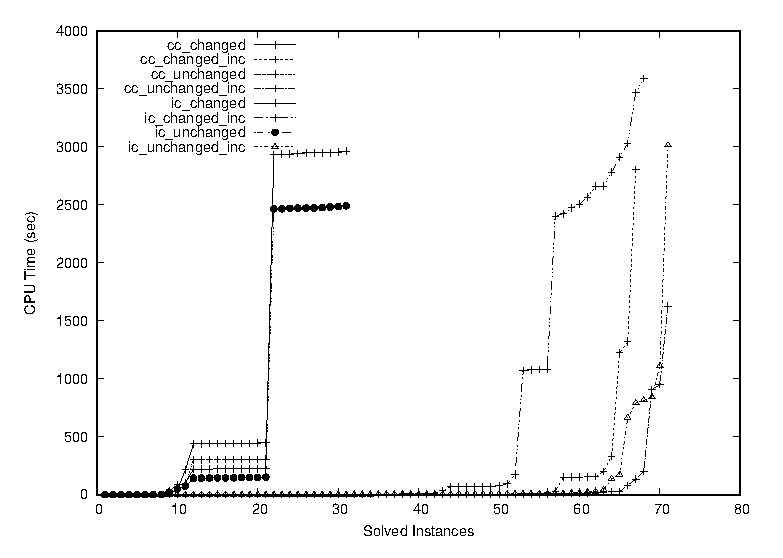
\includegraphics[scale=0.6]{fig/cactus.eps}
  \end{figure}

  \begin{itemize}
    \item 改良ソルバーは基本ソルバーより多くの問題を高速に解いている.
    \item \code{unchanged}符号化は\code{changed}符号化より多くの問題を高速に解いている.
  \end{itemize}
  
\end{frame}

%%%%%%%%%%%%%%%%%%%%%%%%%%%%%%%%%%%%%%%%%%%%%%%%%%
%% 今後の課題
%%%%%%%%%%%%%%%%%%%%%%%%%%%%%%%%%%%%%%%%%%%%%%%%%%

\begin{frame}\frametitle{まとめと今後の課題}

  \begin{block}{まとめ}
    \begin{itemize}
      \item 有界組合せ遷移を提案した.
      \item 有界組合せ遷移を解く2つのソルバーを提案した.
      \begin{itemize}
        \item 特に改良ソルバーは{\clingo}の PythonAPI を用いて高速化を図っている.
      \end{itemize}
      \item $k$彩色遷移問題を解く二つの符号化を提案した.
      \item 独自に作成したベンチマーク問題を用い,2つのソルバー及び2つの符号化の評価
            実験を行った.
      \begin{itemize}
        \item 実験の結果,改良ソルバーの優位性が確かめられた.
      \end{itemize}
    \end{itemize}
  \end{block}
  
  \begin{alertblock}{今後の課題}
    \begin{itemize}
      \item 改良ソルバーの高速化.
      \item 組合せ遷移問題の記述例の蓄積.
      \item $k$彩色遷移問題の ASP 符号化の高速化.
    \end{itemize}
  \end{alertblock}

\end{frame}

%###########################################################
%##### 補助スライド ########################################
%###########################################################

%%%% 補助スライド
\appendix
\backupbegin

\begin{frame}{~}
 \centering
 - 補足用 -
\end{frame} 

%%%%%%%%%%%%%%%%%%%%%%%%%%%%%%%%%%%%%%%%%%%%%%%%%%
%% 電気制約
%%%%%%%%%%%%%%%%%%%%%%%%%%%%%%%%%%%%%%%%%%%%%%%%%%
\begin{frame}{補足 : 電気制約}
 \begin{itemize}
  \item \alert{電気制約}は,送電する電流$\cdot$電圧の適正範囲を保証する制約.
  \begin{itemize}
   \item 供給経路の各区間で許容電流を超えない.
   \item 電気抵抗による電圧降下が許容範囲を超えない.
   \item etc.
  \end{itemize}
  \item 電流と電圧が影響し合う\structure{実数ドメイン上の制約}によって表される.
		% \begin{itemize}
		%  		 \item 送電システム上の条件など.
		% \end{itemize}
  \item 実数ドメイン上の制約は,純粋なASPのみで扱うのは\alert{困難}.
		\begin{itemize}
		 \item 緩和問題として,変電所から供給できる家庭の数に上限をつける.
		 \item ASPMT技術により,ASPで得られた解について,
			   背景理論ソルバーと連携して実数ドメイン上の制約を調べる.
		\end{itemize}
 \end{itemize}
\end{frame}

%%%%%%%%%%%%%%%%%%%%%%%%%%%%%%%%%%%%%%%%%%%%%%%%%%
%% 基礎化
%%%%%%%%%%%%%%%%%%%%%%%%%%%%%%%%%%%%%%%%%%%%%%%%%%
\begin{frame}{補足 : ASPシステム}
 
 \vspace{-0.5cm}

 \begin{figure}[htbp]
  \centering
  %%%%%%%%%%%%%%%%%%%%%%%%%%%%%%%%%%%%%%%%%%%%%%%%%%
%% 基礎化の流れの図
%%%%%%%%%%%%%%%%%%%%%%%%%%%%%%%%%%%%%%%%%%%%%%%%%%
\begin{tikzpicture}

 \definecolor{edge}{RGB}{38,38,134}
 \definecolor{node}{RGB}{220,220,249}

 \definecolor{alert_edge}{RGB}{191,0,0}
 \definecolor{alert_node}{RGB}{249,200,200}

 \definecolor{ex_edge}{RGB}{0,96,0}
 \definecolor{ex_node}{RGB}{230,239,230}

 \def\nodespace{2.4cm}

 \tikzset{block/.style={rectangle, thick, draw=edge, fill=node, text width=3cm, 
 text centered, rounded corners, text width=2cm, minimum height=1.5cm}};

 \tikzset{alertblock/.style={rectangle, thick, draw=alert_edge, fill=alert_node, 
 text width=3cm, text centered, rounded corners, text width=1.5cm, minimum height=1.2cm}};

 \node[block](ikkai){一階ASP\\プログラム};

 \node[rectangle,rounded corners, thick, draw=ex_edge, fill=ex_node, 
 right=0.22*\nodespace of ikkai, minimum width=6cm, minimum height=3cm, 
 text centered, label=ASPシステム](sys){};

 \node[block, right=\nodespace of ikkai](meidai){命題ASP\\プログラム};
 \node[block, right=\nodespace of meidai](ASP){解集合};

 \node[right=0.6*\nodespace of ikkai, text width=1.5cm, 
 text centered, text=red, anchor=south](){基礎化\\ソルバー};
 \node[right=0.4*\nodespace of meidai, text width=1.5cm, 
 text centered, text=red, anchor=south](){解集合\\ソルバー};

 
 \foreach \u / \v / \n in {ikkai/meidai,meidai/ASP}
 \draw [thick,->] (\u) to (\v);

\end{tikzpicture}
 \end{figure}

 \vspace{-0.5cm}

 \begin{exampleblock}{}
  \begin{enumerate}
   \item 一階ASPプログラムを基礎化ソルバーによって,
		 命題ASPプログラムに\alert{基礎化}する.
   \item 命題ASPプログラムについて,SAT技術を応用した解集合ソルバーが解集合を探索する.
  \end{enumerate}
 \end{exampleblock}

\end{frame}
%%%%%%%%%%%%%%%%%%%%%%%%%%%%%%%%%%%%%%%%%%%%%%%%%%
%% ASPの構文
%%%%%%%%%%%%%%%%%%%%%%%%%%%%%%%%%%%%%%%%%%%%%%%%%%
\begin{frame}{ASPの構文}
  \begin{alertblock}{}\centering
    ASPの言語は論理プログラムをベースとしている~\footnotemark.
  \end{alertblock}
  \begin{itemize}
  \item \structure{\bf 論理プログラム}とは,以下の\structure{\bf ルール}の有限集合である.
    \begin{center}
      \begin{minipage}[c]{0.7\textwidth}
        \begin{block}{}\centering
          $a_0$\quad\code{:-}\quad$a_1$\code{,}\ldots\code{,}$a_m$\code{,}
          \ \code{not}~$a_{m+1}$\code{,}\ldots\code{,} \code{not}~$a_n$\code{.}
        \end{block}        
      \end{minipage}
   \end{center}\vfill
    $0 \leq m \leq n$ であり,各 $a_i$ はアトム,
    \code{not}は\structure{\bf デフォルトの否定},\\
    ``\code{,}''は連言(AND)を表す.``\code{:-}''の左辺を\structure{\bf ヘッド},
		右辺を\structure{\bf ボディ}と呼ぶ.
  \item \alert{\bf 直感的な意味}は,
    「$a_1,\ldots,a_m$がすべて成り立ち,
    $a_{m+1},\ldots,a_n$のそれぞれが成り立たないならば,
    $a_0$が成り立つ」である.
  \item ボディが空のルールを\structure{\bf ファクト}と呼び,``\code{:-}''は省略できる.
  \item ヘッドが空のルールを\structure{\bf 一貫性制約}と呼ぶ.例えば,\hspace{-1ex}
    ``\code{:-} $a_1$\code{,} \code{not}~$a_{2}$''は,
    「$a_1$が成り立つならば,$a_2$が成り立つ」を意味する.
  \end{itemize}
  \footnotetext{本発表では標準論理プログラムを単に論理プログラムと呼ぶ.}
\end{frame}
%%%%%%%%%%%%%%%%%%%%%%%%%%%%%%%%%%%%%%%%%%%%%%%%%%
%% ASPの拡張構文
%%%%%%%%%%%%%%%%%%%%%%%%%%%%%%%%%%%%%%%%%%%%%%%%%%
\begin{frame}{ASPの拡張構文}
\begin{alertblock}{}\centering
  組合せ問題を解くための便利な構文が用意されている.
\end{alertblock}
\begin{itemize}
 \item \structure{\bf 選択子}
   \begin{center}
     \code{\{}$a_1$\code{;}\ldots\code{;}$a_n$\code{\}}
   \end{center}
   アトム集合 $\{a_1,\dots,a_n\}$
   の任意の部分集合が成り立つことを意味する.
 \item \structure{\bf 個数制約}
   \begin{center}
     $lb$\ \code{\{}$a_1$\code{;}\ldots\code{;}$a_n$\code{\}}\ $ub$
   \end{center}
   $a_1,\dots,a_n$ のうち,
   $lb$個以上,$ub$個以下が成り立つことを意味する.
 \item \structure{\bf 重み付き個数制約}
   \begin{center}
     $lb$ \code{\#sum\{} $w_1$\code{:}$a_1$\code{;}\ldots\code{;}$w_n$\code{:}$a_n$ \code{\}} $ub$
   \end{center}
   $a_1,\dots,a_n$のうち,
   成り立つアトムの重み和が$lb$以上,$ub$以下になることを意味する.
\end{itemize}
\end{frame}
%%%%%%%%%%%%%%%%%%%%%%%%%%%%%%%%%%%%%%%%%%%%%%%%%%
%% 改良符号化 (到達可能性)
%%%%%%%%%%%%%%%%%%%%%%%%%%%%%%%%%%%%%%%%%%%%%%%%%%
\begin{frame}[fragile]{改良符号化: 到達可能性}
\begin{exampleblock}{}\small
\begin{lstlisting}
(1) { inForest(X,Y) } :- edge(X,Y).
\end{lstlisting}
\end{exampleblock}
\begin{itemize}
 \item (1) 各辺\code{(X,Y)について},根付き全域森に含まれること意味する \\
	  アトム\code{inForest(X,Y)}を導入する.
\end{itemize}
\begin{exampleblock}{}\small
\begin{lstlisting}
(2) reached(R,R) :- root(R).
(3) reached(X,R) :- reached(Y,R), inForest(Y,X).
(4) reached(X,R) :- reached(Y,R), inForest(X,Y).
\end{lstlisting}
\end{exampleblock}
\vfill
\begin{itemize}
\item アトム\code{reached(X,R)}は,ノード\code{X}が根ノード\code{R}から到達可能であることを意味する.
%\item (2) 各根ノード\code{R}について,自分自身から到達可能であることを表す.
\item (3) ノード\code{Y}が根ノード\code{R}から到達可能かつ,辺\code{(Y,X)}が根付き全域森に含まれるならば,
	  ノード\code{X}も同じ根ノード\code{R}から到達可能であることを表す.
\end{itemize}
\end{frame}
%%%%%%%%%%%%%%%%%%%%%%%%%%%%%%%%%%%%%%%%%%%%%%%%%%
%% 改良符号化 (根付き連結制約)
%%%%%%%%%%%%%%%%%%%%%%%%%%%%%%%%%%%%%%%%%%%%%%%%%%
\begin{frame}[fragile]{改良符号化: 根付き連結制約}
\begin{exampleblock}{}\small
\begin{lstlisting}
(5) :- node(X), not 1 { reached(X,R) } 1.
\end{lstlisting}
\end{exampleblock}
\vfill
\begin{itemize}
\item (5) 各ノード\code{X}について,ちょうど1つの根からのみ到達可能であることを意味する.
\end{itemize}
\end{frame}
%%%%%%%%%%%%%%%%%%%%%%%%%%%%%%%%%%%%%%%%%%%%%%%%%%
%% 改良符号化 (非閉路制約)
%%%%%%%%%%%%%%%%%%%%%%%%%%%%%%%%%%%%%%%%%%%%%%%%%%
\begin{frame}[fragile]{改良符号化: 非閉路制約}
\begin{minipage}[c]{1.01\textwidth}
\begin{exampleblock}{}\small
\begin{lstlisting}
(6) :- root(R),
       not 1 #sum{ 1,X:reached(X,R) ;
                  -1,X,Y:inForest(X,Y),reached(X,R),reached(Y,R)
                 } 1.
\end{lstlisting}
\end{exampleblock}
\end{minipage}
\vfill
\begin{itemize}
\item (6) 各連結成分の\structure{\bf ノード数と辺数の差が1}になることを意味する.
\item 各連結成分が\structure{\bf 木の性質}を満たすことにより,サイクルを持たない
	  ことを保証する.
\end{itemize}
\end{frame}
%%%%%%%%%%%%%%%%%%%%%%%%%%%%%%%%%%%%%%%%%%%%%%%%%%
%% ルール数の比較
%%%%%%%%%%%%%%%%%%%%%%%%%%%%%%%%%%%%%%%%%%%%%%%%%%
\begin{frame}{基礎化後のルール数}
  \begin{itemize}
  \item グラフのノード数を$|V|$,根ノードの数を$|R|$とする.
  \end{itemize}
  \begin{table}[t]
    \centering
    %%%%%%%%%%%%%%%%%%%%%%%%%%%%%%%%%%%%%%%%%%%%%%%%%%%%%%%%%%%%%%%%
\chapter{ハミルトン閉路問題および関連問題のASP符号化}\label{chap:proposal}
%%%%%%%%%%%%%%%%%%%%%%%%%%%%%%%%%%%%%%%%%%%%%%%%%%%%%%%%%%%%%%%% 

%%%%
\begin{figure}[h]
  \centering
  \thicklines
  \setlength{\unitlength}{1.2pt}
  \small\footnotesize\scriptsize
  \begin{picture}(280,57)(4,-10)
    \put(  0, 20){\dashbox(50,24){\shortstack{HCP問題\\インスタンス}}}
    \put( 60, 20){\framebox(50,24){変換器}}
    \put(120, 20){\dashbox(50,24){\shortstack{ASPファクト}}}
    \put(120,-10){\dashbox(50,24){\shortstack{ASP符号化\\(論理プログラム)}}}
    \put(180, 20){\framebox(50,24){ASPシステム}}
    \put(240, 20){\dashbox(50,24){\shortstack{HCP問題\\の解}}}
    \put( 50, 32){\vector(1,0){10}}
    \put(110, 32){\vector(1,0){10}}
    \put(170, 32){\vector(1,0){10}}
    \put(230, 32){\vector(1,0){10}}
    \put(170, +2){\line(1,0){4}}
    \put(174, +2){\line(0,1){30}}
  \end{picture}  
\caption{ASP を用いたハミルトン閉路問題(HCP)の解法}
\label{fig:arch}
\end{figure}
%%%%

%\begin{figure}[tbp]
\tikz{
  %1ノード目
  \path[draw=black, fill=blue!20, rounded corners=5pt]%線の設定
  node[at={(0.75,0.75)}] {問題}%文字を入れる
  (0,0) --(1.5,0) --(1.5,1.5) --(0,1.5) --cycle;%外周
  %2ノード目
  \path[draw=black, fill=blue!20, rounded corners=5pt, shift={(3,0)}]
  node[at={(0.75,0.75)}] {
    \begin{tabular}{c}
      ASP\\
      ファクト
    \end{tabular}
  }
  (0,0) --(1.5,0) --(1.5,1.5) --(0,1.5) --cycle;
  %3ノード目文字が複数行
  \path[draw=black, fill=green!20, rounded corners=5pt, shift={(6,0)}]
  node[at={(0.75,0.75)}] {
    \begin{tabular}{c}
      ASP\\
      システム
    \end{tabular}
  }
  (0,0) --(1.5,0) --(1.5,1.5) --(0,1.5) --cycle;
  %4ノード目文字が複数行
  \path[draw=black, fill=blue!20, rounded corners=5pt, shift={(9,0)}]
  node[at={(0.75,0.75)}] {解集合}
  (0,0) --(1.5,0) --(1.5,1.5) --(0,1.5) --cycle;
  %5ノード目文字が複数行
  \path[draw=black, fill=red!20, rounded corners=5pt, shift={(3,-3)}]
  node[at={(0.75,0.75)}] {
    \begin{tabular}{c}
      ASP\\
      符号化
    \end{tabular}
  }
  (0,0) --(1.5,0) --(1.5,1.5) --(0,1.5) --cycle;
  \draw[arrows=->] (1.5,0.75) --(3.0,0.75);
  \draw[arrows=->,shift={(3,0)}] (1.5,0.75) --(3.0,0.75);
  \draw[arrows=->,shift={(6,0)}] (1.5,0.75) --(3.0,0.75);
  \draw[arrows=->] (4.5,-2.25) --(6.0,0.5);
}
\caption{ASPを用いた解法}
\label{aspmethod}
\end{figure}


ASP を用いたハミルトン閉路問題および関連問題の解法について述べる.
図~\ref{fig:arch}に,解法の流れを示す.
与えられたハミルトン閉路問題は ASP ファクトに変換され,
ハミルトン閉路問題を解く ASP 符号化と結合され,
ASP システムによって解が計算される.
本論文では,ASP システムとして{\clingo}を用いる.

%%%%%%%%%%%%%%%%%%%%%%%%%%%%%%%%%%%%%%%%%%%%%%%%%%%%%%%%%%%%%%%%%%%%%%%
\section{ASPファクト形式}
%%%%%%%%%%%%%%%%%%%%%%%%%%%%%%%%%%%%%%%%%%%%%%%%%%%%%%%%%%%%%%%%%%%%%%%

%%%%%%%%%%%%%%%%%%%%%%%%%%%%%%
\begin{figure}[t]
\begin{center}
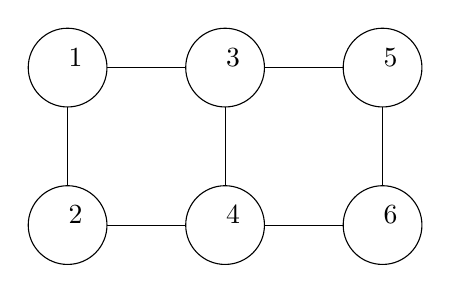
\begin{tikzpicture}
  %ノード1  
  \draw(4,2) circle (0.5)
  node[at={(4.1,2.1)}] {
    \begin{tabular}{c}
      1
    \end{tabular}
  };
  %ノード2  
  \draw(4,0) circle (0.5)
  node[at={(4.1,0.1)}] {
    \begin{tabular}{c}
      2
    \end{tabular}
  };
  %ノード3  
  \draw(6,2) circle (0.5)
  node[at={(6.1,2.1)}] {
    \begin{tabular}{c}
      3
    \end{tabular}
  };
  %ノード4  
  \draw(6,0) circle (0.5)
  node[at={(6.1,0.1)}] {
    \begin{tabular}{c}
      4
    \end{tabular}
  };
  %ノード5  
  \draw(8,2) circle (0.5)
  node[at={(8.1,2.1)}] {
    \begin{tabular}{c}
      5
    \end{tabular}
  };
  %ノード6  
  \draw(8,0) circle (0.5)
  node[at={(8.1,0.1)}] {
    \begin{tabular}{c}
      6
    \end{tabular}
  };
\draw(4,0.5) --(4,1.5);
\draw(6,0.5) --(6,1.5);
\draw(8,0.5) --(8,1.5);
\draw(4.5,0) --(5.5,0);
\draw(4.5,2) --(5.5,2);
\draw(6.5,0) --(7.5,0);
\draw(6.5,2) --(7.5,2);
\end{tikzpicture}

\caption{入力となる重み付き無向グラフの例}
\label{graphexample}
\end{center}
\end{figure}
%%%%%%%%%%%%%%%%%%%%%%%%%%%%%%

%%%%%%%%%%%%%%%%%%%%%%%%%%%%%%
\lstinputlisting[float=t,caption={%
図~\ref{graphexample}のASPファクト表現},%
captionpos=b,frame=single,label=code:graph_example.lp,%
numbers=none,%
breaklines=true,%
columns=fullflexible,keepspaces=true,%
basicstyle=\ttfamily\scriptsize]{code/graph_example.lp}
%%%%%%%%%%%%%%%%%%%%%%%%%%%%%%


本節では,最短ハミルトン閉路問題の例にとって,
入力となる重み付き無向グラフ(図~\ref{graphexample})の
ASP ファクト形式について説明する.
%
このグラフは,頂点数が6,辺の数が7であり,辺に付けられた値は距離を表す.
コード~\ref{code:graph_example.lp}に,ASPファクト形式を示す.
%
アトム\code{node/1}は頂点,\code{edge/2}は辺,\code{cost/3}は距離を表す.
例えば,\code{cost(1,2,3)}は,辺\code{edge(1,2)}の距離が3であることを
表している.

%%%%%%%%%%%%%%%%%%%%%%%%%%%%%%%%%%%%%%%%%%%%%%%%%%%%%%%%%%%%%%%%%%%%%%%
\section{ハミルトン閉路問題の ASP 符号化}\label{hamiltonianasp}
%%%%%%%%%%%%%%%%%%%%%%%%%%%%%%%%%%%%%%%%%%%%%%%%%%%%%%%%%%%%%%%%%%%%%%%

ハミルトン閉路問題は,与えられたグラフの全頂点をちょうど一度ずつ通る閉
路(ハミルトン閉路)が存在するかどうかを判定する問題である.
$G=(V,E)$にハミルトン閉路が存在する必要十分条件は,
以下の2つの制約を満たす部分グラフ$G'=(V,E')$が存在することである.

\begin{itemize}
\item $G'$の各頂点の次数が2 (次数制約)
\item $G'$が連結である (連結制約)
\end{itemize}

本論文では,前者を\textbf{次数制約},後者を\textbf{連結制約}と呼ぶ.
ハミルトン路問題は,ハミルトン閉路問題から始点と終点が一致するという閉
路の条件を取り除いたものである.
ハミルトン路問題では,次数制約は以下のように変わる.

\begin{itemize}
\item 始点と終点の次数が1,他の頂点の次数が2
\end{itemize}

以下では,ハミルトン閉路問題に対する3つの ASP 符号化
\textsf{undirected},\textsf{directed},\textsf{acyclicity}
を提案する.

%%%%%%%%%%%%%%%%%%%%%%%%%%%%%%%%%%%%%%%%%%%%%%%%%%%%%%%%%%%%%%%%%%%%%%%
\subsection{\textsf{undirected}符号化}
%%%%%%%%%%%%%%%%%%%%%%%%%%%%%%%%%%%%%%%%%%%%%%%%%%%%%%%%%%%%%%%%%%%%%%%

%%%%%%%%%%%%%%%%%%%%%%%%%%%%%%
\lstinputlisting[float=t,caption={%
\textsf{undirected}符号化},%
captionpos=b,frame=single,label=code:hamilton1.lp,%
numbers=left,%
breaklines=true,%
columns=fullflexible,keepspaces=true,%
basicstyle=\ttfamily\footnotesize]{code/hamilton1.lp}
%%%%%%%%%%%%%%%%%%%%%%%%%%%%%%

\textsf{undirected}符号化は,ハミルトン閉路問題の次数制約と連結制約を,
ASP の一貫性制約で表した基本的な符号化である.
コード~\ref{code:hamilton1.lp}に,\textsf{undirected}符号化を示す.
この符号化は,ハミルトン閉路問題とハミルトン路問題の両方に対応している.
符号化中の\code{s}は始点の頂点番号,\code{t}は終点の頂点番号を表し,こ
れらは実行時に与えられる.
ここでは,ハミルトン閉路問題(\code{s}=\code{t})の場合について説明する.

\begin{itemize}
\item 1行目のルールは,各辺\code{edge(X,Y)}に対して,その辺がハミルト
  ン閉路に含まれるかどうかを意味するアトム\code{in(X,Y)}を選択子を用い
  て導入している.
\item 次数制約は3行目のルールで表される.このルールは,
  各頂点\code{node(X)}に対して,その次数の和が2に等しいことを個数制約
  を使って表している.
\item 連結制約は11行目のルールで表される.
ある頂点\code{X}が始点\code{s}から到達可能であることを意味する補助アト
ム\code{reached(X)}を導入する.
8行目のルールは,始点\code{s}が到達可能あることを表している.
9行目のルールは,各辺\code{X}--\code{Y}に対して,その辺がハミルトン閉
路に含まれ(\code{in(X,Y)}),かつ,頂点\code{X}が始点から到
達可能であれば(\code{reached(X)}),\code{Y}も到達可能であることを表している.
10行目は9行目と同様であるが,辺\code{Y}--\code{X}の場合を表している.
11行目のルールは,各頂点\code{node(X)}が始点から到達可能でなければな
らないことを一貫性制約を使って表している.
\end{itemize}

%%%%%%%%%%%%%%%%%%%%%%%%%%%%%%%%%%%%%%%%%%%%%%%%%%%%%%%%%%%%%%%%%%%%%%%
\subsection{\textsf{directed}符号化}
%%%%%%%%%%%%%%%%%%%%%%%%%%%%%%%%%%%%%%%%%%%%%%%%%%%%%%%%%%%%%%%%%%%%%%%

%%%%%%%%%%%%%%%%%%%%%%%%%%%%%%
\lstinputlisting[float=t,caption={%
\textsf{directed}符号化},%
captionpos=b,frame=single,label=code:hamilton2.lp,%
numbers=left,%
breaklines=true,%
columns=fullflexible,keepspaces=true,%
basicstyle=\ttfamily\footnotesize]{code/hamilton2.lp}
%%%%%%%%%%%%%%%%%%%%%%%%%%%%%%

\textsf{directed}符号化は,\textsf{undirected}符号化をベースに,
与えられた無向グラフの各辺$u-v$に対して,2つの弧$u\rightarrow v$と
$v\rightarrow u$を対応させることで有向グラフ化して解く符号化である.
コード~\ref{code:hamilton2.lp}に,\textsf{directed}符号化を示す.
前節と同様に,ハミルトン閉路問題(\code{s}=\code{t})の場合について説明する.

\begin{itemize}
\item 1行目では,無向グラフの有向グラフ化を行う.
  与えられた無向グラフの各辺\code{edge(X,Y)}に対して,
  2つの弧\code{edge(X,Y)},\code{edge(Y,X)}を導入した.
\item 2行目のルールは,各弧\code{edge(X,Y)}に対して,その弧がハミルト
  ン閉路に含まれるかどうかを意味するアトム\code{in(X,Y)}を選択子を用い
  て導入している.
\item 次数制約は4,5行目のルールで表される.
  4行目では,各頂点\code{node(X)}に対して,
  その出次数が1に等しいことを個数制約を使って表している.
  5行目では,入次数について4行目と同様の制約を表す.
\item 連結制約は15行目のルールで表される.
  ある頂点\code{X}が始点\code{s}から到達可能であることを意味する
  補助アトム\code{reached(X)}を導入する.
  13行目のルールは,始点\code{s}が到達可能あることを表している.
  14行目のルールは,各弧\code{X}--\code{Y}に対して,その弧がハミルトン閉路
  に含まれ(\code{in(X,Y)}),かつ,頂点\code{X}が始点から
  到達可能であれば(\code{reached(X)}),\code{Y}も到達可能であることを表している.
  15行目のルールは,各頂点\code{node(X)}が始点から到達可能でなければ
  ならないことを一貫性制約を使って表している.
\item 18行目のルールは,解についての対称性を除去する.
  与えられた無向グラフ上の各ハミルトン閉路に対して,
  それを変換した有向グラフ上のハミルトン閉路は対称な2つが存在する.
  これによる解の重複を防ぐために,18行目のルールは,各弧\code{s}--\code{X},
  \code{Y}--\code{s}がハミルトン閉路に含まれるならば(\code{in(s,X),in(Y,s)}),
  \code{X < Y}でなければならないことを,一貫性制約を用いて表している
\end{itemize}

%%%%%%%%%%%%%%%%%%%%%%%%%%%%%%%%%%%%%%%%%%%%%%%%%%%%%%%%%%%%%%%%%%%%%%%
\subsection{\textsf{acyclicity}符号化}
%%%%%%%%%%%%%%%%%%%%%%%%%%%%%%%%%%%%%%%%%%%%%%%%%%%%%%%%%%%%%%%%%%%%%%%

%%%%%%%%%%%%%%%%%%%%%%%%%%%%%%
\lstinputlisting[float=t,caption={%
\textsf{acyclicity}符号化},%
captionpos=b,frame=single,label=code:hamilton3.lp,%
numbers=left,%
breaklines=true,%
columns=fullflexible,keepspaces=true,%
basicstyle=\ttfamily\footnotesize]{code/hamilton3.lp}
%%%%%%%%%%%%%%%%%%%%%%%%%%%%%%

\textsf{acyclicity}符号化は,\textsf{directed}符号化をベースに,
連結の制約に代わる部分閉路禁止制約を組込み非閉路制約で表現した符号化である.
コード~\ref{code:hamilton3.lp}に,\textsf{acyclicity}符号化を示す.
前節と同様に,ハミルトン閉路問題(\code{s}=\code{t})の場合について説明する.

\begin{itemize}
\item 1行目では,無向グラフの有向グラフ化を行う.
  与えられた無向グラフの各辺\code{edge(X,Y)}に対して,
  2つの弧\code{edge(X,Y)},\code{edge(Y,X)}を導入した.
\item 2行目のルールは,各弧\code{edge(X,Y)}に対して,その弧がハミルト
  ン閉路に含まれるかどうかを意味するアトム\code{in(X,Y)}を選択子を用い
  て導入している.
\item 次数制約は4,5行目のルールで表される.
  4行目では,各頂点\code{node(X)}に対して,
  その出次数が1に等しいことを個数制約を使って表している.
  5行目では,入次数について4行目と同様の制約を表す.
\item 部分閉路禁止制約は14行目のルールで表される.
  このルールは,始点でない各頂点\code{X},\code{Y}について,
  弧\code{X}--\code{Y}がハミルトン閉路に含まれるならば(\code{in(X,Y)}),
  そのような弧の集合をもつグラフが閉路をもたないことを,\code{#edge}宣言を用いて表す.
  ようするに,始点(終点)を含まないような閉路を禁止している.
\item 17行目のルールは,解についての対称性を除去する.
  与えられた無向グラフ上の各ハミルトン閉路に対して,
  それを変換した有向グラフ上のハミルトン閉路は対称な2つが存在する.
  これによる解の重複を防ぐために,17行目のルールは,各弧\code{s}--\code{X},
  \code{Y}--\code{s}がハミルトン閉路に含まれるならば(\code{in(s,X),in(Y,s)}),
  \code{X < Y}でなければならないことを,一貫性制約を用いて表している
\end{itemize}

%%%%%%%%%%%%%%%%%%%%%%%%%%%%%%%%%%%%%%%%%%%%%%%%%%%%%%%%%%%%%%%%%%%%%%% 
\section{最短ハミルトン閉路問題のASP符号化}\label{minexpl}
%%%%%%%%%%%%%%%%%%%%%%%%%%%%%%%%%%%%%%%%%%%%%%%%%%%%%%%%%%%%%%%%%%%%%%% 

%% %%%%%%%%%%%%%%%%%%%%%%%%%%%%%%
%% \lstinputlisting[caption =  最適化,label = minimize]{code/obj_minimize.lp}
%% %%%%%%%%%%%%%%%%%%%%%%%%%%%%%%

%%%%%%%%%%%%%%%%%%%%%%%%%%%%%%
\lstinputlisting[float=t,caption={%
最小化},%
captionpos=b,frame=single,label=code:obj_minimize.lp,%
numbers=left,%
breaklines=true,%
columns=fullflexible,keepspaces=true,%
basicstyle=\ttfamily\footnotesize]{code/obj_minimize.lp}
%%%%%%%%%%%%%%%%%%%%%%%%%%%%%%

最短ハミルトン閉路問題の目的関数は,
ハミルトン閉路を構成する各辺の距離の総和である.
コード\ref{code:obj_minimize.lp}は,
その目的関数の最小化を表す.
このコードは,各辺\code{edge(X,Y)}に対して,その辺がハミルトン閉路に
含まれ(\code{in(X,Y)}),その距離が\code{C}である時に(\code{cost(X,Y,C)}),
\code{C}の総和の最小化を,最小化関数を用いて表している.
.
%%%%%%%%%%%%%%%%%%%%%%%%%%%%%%
\lstinputlisting[float=t,caption={%
重み付き無向グラフの有向グラフ化},%
captionpos=b,frame=single,label=code:cost_both.lp,%
numbers=left,%
breaklines=true,%
columns=fullflexible,keepspaces=true,%
basicstyle=\ttfamily\footnotesize]{code/cost_both.lp}
%%%%%%%%%%%%%%%%%%%%%%%%%%%%%%

符号化directed,acyclicityについては,
与えられた無向グラフの各辺\code{edge(X,Y)}に対して,
2つの弧\code{edge(X,Y)},\code{edge(Y,X)}を導入した.
各辺の距離もこれに対応させるために,コード\ref{code:cost_both.lp}
を追加した.
このルールは,各辺\code{X}--\code{Y}の距離を表す\code{cost(X,Y,C)}について,
\code{cost(Y,X,C)}を導入する.
これにより,与えられた無向グラフの各辺\code{edge(X,Y)}の重み\code{C}が
2つの弧\code{edge(X,Y)},\code{edge(Y,X)}にも付与された.

%%%%%%%%%%%%%%%%%%%%%%%%%%%%%%%%%%%%%%%%%%%%%%%%%%%%%%%%%%%%%%%%%%%%%%% 
\section{コスト制約付きハミルトン閉路のASP符号化}
%%%%%%%%%%%%%%%%%%%%%%%%%%%%%%%%%%%%%%%%%%%%%%%%%%%%%%%%%%%%%%%%%%%%%%% 

%%%%%%%%%%%%%%%%%%%%%%%%%%%%%%
\lstinputlisting[float=t,caption={%
コスト制約},%
captionpos=b,frame=single,label=code:cost_constraint.lp,%
numbers=left,%
breaklines=true,%
columns=fullflexible,keepspaces=true,%
basicstyle=\ttfamily\footnotesize]{code/cost_constraint.lp}
%%%%%%%%%%%%%%%%%%%%%%%%%%%%%%

コスト制約付きハミルトン閉路問題は
ハミルトン閉路問題に,距離の総和が所与の閾値以下 (または以上) であること
を制約条件として付加した問題である.
コード\ref{code:const_constraing.lp}のルールは,その制約を表す.
ルール中の\code{c}は閾値を表し,これは実行時に与えられる.
このルールは,各辺\code{edge(X,Y)}に対して,その辺がハミルトン閉路に
含まれ(\code{in(X,Y)}),その距離が\code{C}である時に(\code{cost(X,Y,C)}),
\code{C}の総和が\code{c}以下でなければならないことを,
一貫性制約と重み付き個数制約を用いて表す.

また,\ref{minexpl}と同様に,
符号化directed,acyclicityについては,
アトム\code{cost}についても有向グラフ化に
対応させるためにコード\ref{code:cost_both.lp}を追加した.
%%%%%%%%%%%%%%%%%%%%%%%%%%%%%%%%%%%%%%%%%%%%%%%%%%%%%%%%%%%%%%%%%%%%%%%

%%% Local Variables:
%%% mode: latex
%%% TeX-master: "paper"
%%% End:

  \end{table}
\end{frame}

%%%%%%%%%%%%%%%%%%%%%%%%%%%%%%%%%%%%%%%%%%%%%%%%%%
%% ASPのコード
%%%%%%%%%%%%%%%%%%%%%%%%%%%%%%%%%%%%%%%%%%%%%%%%%%
\begin{frame}[fragile]{補足 : 根付き全域森 基本符号化}
%%%%%%%%%%%%%%%%%%%%%%%%%%%%%%%%% 
\lstinputlisting[frame=single,label=code:roop,%
xleftmargin=1zw,%
xrightmargin=1zw,%
numbersep=5pt,%
numbers=left,%
breaklines=true,%
columns=fullflexible,keepspaces=true,%
basicstyle=\ttfamily\scriptsize]{code/srf1.lp}
%%%%%%%%%%%%%%%%%%%%%%%%%%%%%%%%%
\end{frame}

\begin{frame}[fragile]{補足 : 遷移問題 シングルショット符号化}

\begin{multicols*}{2}
%%%%%%%%%%%%%%%%%%%%%%%%%%%%%%%%% 
\lstinputlisting[frame=single,label=code:roop,%
xleftmargin=1zw,%
xrightmargin=1zw,%
numbersep=5pt,%
numbers=left,%
breaklines=true,%
columns=fullflexible,keepspaces=true,%
basicstyle=\ttfamily\tiny]{code/trans-const.lp}
%%%%%%%%%%%%%%%%%%%%%%%%%%%%%%%%%
\end{multicols*}
\end{frame}

\begin{frame}[fragile]{補足 : 遷移問題 マルチショット符号化}
\begin{multicols*}{2}
%%%%%%%%%%%%%%%%%%%%%%%%%%%%%%%%%
\lstinputlisting[frame=single,label=code:incmode,% 
xleftmargin=1zw,%
xrightmargin=1zw,%
numbersep=5pt,%
numbers=left,%
breaklines=true,%
columns=fullflexible,keepspaces=true,%
basicstyle=\ttfamily\tiny]{code/dnet-trans.lp}
%%%%%%%%%%%%%%%%%%%%%%%%%%%%%%%%% 
\end{multicols*}
\end{frame}

\backupend


\end{document}